\documentclass[sigplan, anonymous, review]{acmart}

\usepackage{algorithm2e}
\DontPrintSemicolon
\SetKwProg{Function}{function}{ do}{end}

\usepackage{listings}
\lstdefinestyle{code}{basicstyle=\ttfamily\footnotesize}
\lstset{style=code}

\newcommand{\draft}[1]{CONTENT HIDDEN FOR REVIEWS}

\keywords{Compiler, Virtual Machine, Dynamic Language, Scheme}

\begin{CCSXML}
  <ccs2012>
  <concept>
  <concept_id>10011007.10011006.10011008.10011009.10011012</concept_id>
  <concept_desc>Software and its engineering~Functional languages</concept_desc>
  <concept_significance>500</concept_significance>
  </concept>
  <concept>
  <concept_id>10011007.10011006.10011041.10010943</concept_id>
  <concept_desc>Software and its engineering~Interpreters</concept_desc>
  <concept_significance>500</concept_significance>
  </concept>
  % <concept>
  % <concept_id>10011007.10010940.10010971.10010564</concept_id>
  % <concept_desc>Software and its engineering~Embedded software</concept_desc>
  % <concept_significance>100</concept_significance>
  % </concept>
  </ccs2012>
\end{CCSXML}

\ccsdesc[500]{Software and its engineering~Functional languages}
\ccsdesc[500]{Software and its engineering~Interpreters}
% \ccsdesc[100]{Software and its engineering~Embedded software}

\begin{document}
\title{Stak Scheme: The tiny R7RS-small implementation}
\author{Yota Toyama}
\email{ytoyama42@gmail.com}

\begin{abstract}
  Small environments for embedded scripting allow software to
  evaluate logic dynamically on resource constrained platforms.
  In this paper, we present Stak Scheme, the tiny R7RS-small
  Scheme implementation.
  The whole interpreter of Stak Scheme contains no more than 10 KLOC as
  its core part is composed of a bytecode compiler written in 1.5 KLOC of Scheme
  and a virtual machine written in 1.5 KLOC of Rust.
  Despite its minimal and naive design, Stak Scheme
  supports all major language features of the R7RS-small standard including
  but not limited to the library system, hygienic macros with
  \texttt{syntax-rules}, continuations, exception handling, and the
  fully-featured \texttt{eval} procedure.
  Our bytecode encoding and decoding algorithms convert code and
  data in bytecode uniformly
  between its in-memory graph format and serialized byte sequences.
  Our evaluation proves that the implementation of Stak Scheme is
  compact compared to the prior work of a small R7RS-small implementation
  whereas its performance is still
  comparable with other implementations of Scheme and the other
  scripting languages despite its minimal design.
\end{abstract}

\maketitle

\section{Introduction}

In the Rust programming language as well as in other system
programming languages, it is cumbersome to evaluate programs
dynamically at runtime. At the same time, bundling large runtimes of
scripting languages into binaries is not always acceptable,
especially on resource constrained platforms, such as embedded systems.

In this paper, we present Stak Scheme, the tiny R7RS-small Scheme
implementation\footnote{
  The implementation of Stak Scheme is available at
  \draft{\url{https://github.com/raviqqe/stak}}. Star me to get in touch!
}.
Following the design of Ribbit Scheme
\cite{ribbit2023}, the tiny and
portable R4RS Scheme implementation, Stak Scheme's virtual machine
achieves reasonable performance and the minimal design
at the same time.
In addition, Stak Scheme supports platforms that do not provide
heap allocations or system APIs\footnote{
  These features correspond to the \texttt{alloc}
  crate (the heap allocation module) and the \texttt{std} crate (the
  system interface module) in Rust's standard library respectively.
}, which enables dynamic scripting in such constrained environments.

We make the following contributions in this paper:

\begin{itemize}
  \item We provide the smallest R7RS-small implementations ever in
    terms of lines of code, which is implemented
    in Scheme and a system programming language.
    The core part of the implementation is composed only of a 1.5 KLOC bytecode
    compiler in Scheme and 1.5 KLOC virtual machine in Rust.
  \item We extend Ribbit Virtual Machine (RVM) from the previous
    work of Ribbit Scheme to build an interpreter compatible with the
    R7RS-small standard on top of it.
    We prove that the architecture of RVM is scalable even when
    loaded with a large chunk of language features and standard
    libraries defined in the R7RS-small standard.
  \item We propose our simple bytecode encoding and decoding algorithms
    alternative to the ones used in Ribbit Scheme, which encodes and
    decodes code and data in bytecode uniformly.
\end{itemize}

The main components of Stak Scheme are split into two.
The first component is a bytecode compiler which compiles source
code in Scheme into bytecode (Section \ref{compiler}).
The other component is a virtual machine which executes the compiled
bytecode (Section \ref{vm}).
In the compiler and the virtual machine, we introduce our simple
bytecode encoding and
decoding algorithms that convert code and data in bytecode
uniformly (Section \ref{bytecode}).
Another interesting trait of Stak Scheme is that the bytecode compiler itself
is an ingredient of the \texttt{(scheme eval)} library.
While compiling given source files, the compiler embeds itself
into the source files (Section \ref{inception}) to build up the library.
Finally, our evaluation demonstrates that the performance of Stak Scheme is
comparable with other Scheme implementations and scripting
languages in spite of its minimal design (Section \ref{evaluation}).

\section{Stak Scheme}

Stak Scheme is a tiny R7RS-small implementation consisting of a
bytecode compiler written in Scheme and a virtual machine written in Rust.
The bytecode compiler compiles Scheme source files and encodes their bytecode
into byte sequences.
The virtual machine decodes the serialized bytecode back into its
in-memory format and executes them.
This split architecture of a bytecode compiler and a virtual machine inherited
from Ribbit Scheme allows us to strip
out unnecessary logic from resulting binaries.
For example, we do not include the logic to parse S-expressions
in the virtual machine.
Instead, we compile and bundle the \texttt{read} procedure which parses
S-expressions in bytecode only if their source files import the
\texttt{(scheme read)} standard library, which contains the
\texttt{read} procedure.
We discuss further details about the design and implementation of the
compiler and virtual machine in Section \ref{compiler} and Section
\ref{vm} respectively.

We design Stak Scheme for two use cases. One is to embed Scheme
programs inside Rust programs as dynamic scripts.
The other is to run standalone Scheme scripts on command lines directly.
For the former use case, we
compile Scheme scripts ahead into bytecode files and include them in
Rust programs by the Cargo build
system\footnote{\url{https://doc.rust-lang.org/cargo/}} so that the
Rust programs can execute them on the virtual machines.
For the latter use case, we
provide a standalone command of \texttt{stak} which runs Scheme script
files given as command line arguments.

Figure \ref{figure:build} shows an example workflow of
embedding a Stak Scheme script into a Rust program.
After a user triggers the \texttt{cargo build} command, which is of the
Cargo build system for Rust, a build
script invokes the \texttt{stak-compile} command of the Stak Scheme
bytecode compiler to compile a Scheme source file \texttt{foo.scm}
(List \ref{list:scheme}) into a bytecode file \texttt{foo.bc}
(List \ref{list:bytecode}).
After that, the Rust compiler \texttt{rustc} compiles a Rust source file
\texttt{main.rs} (List \ref{list:rust}) that includes the bytecode
file to produce the final
executable file.

\begin{figure}
  \begin{center}
    \caption{Workflow of embedding Stak Scheme in Rust}
    \label{figure:build}
    \vspace{1em}
    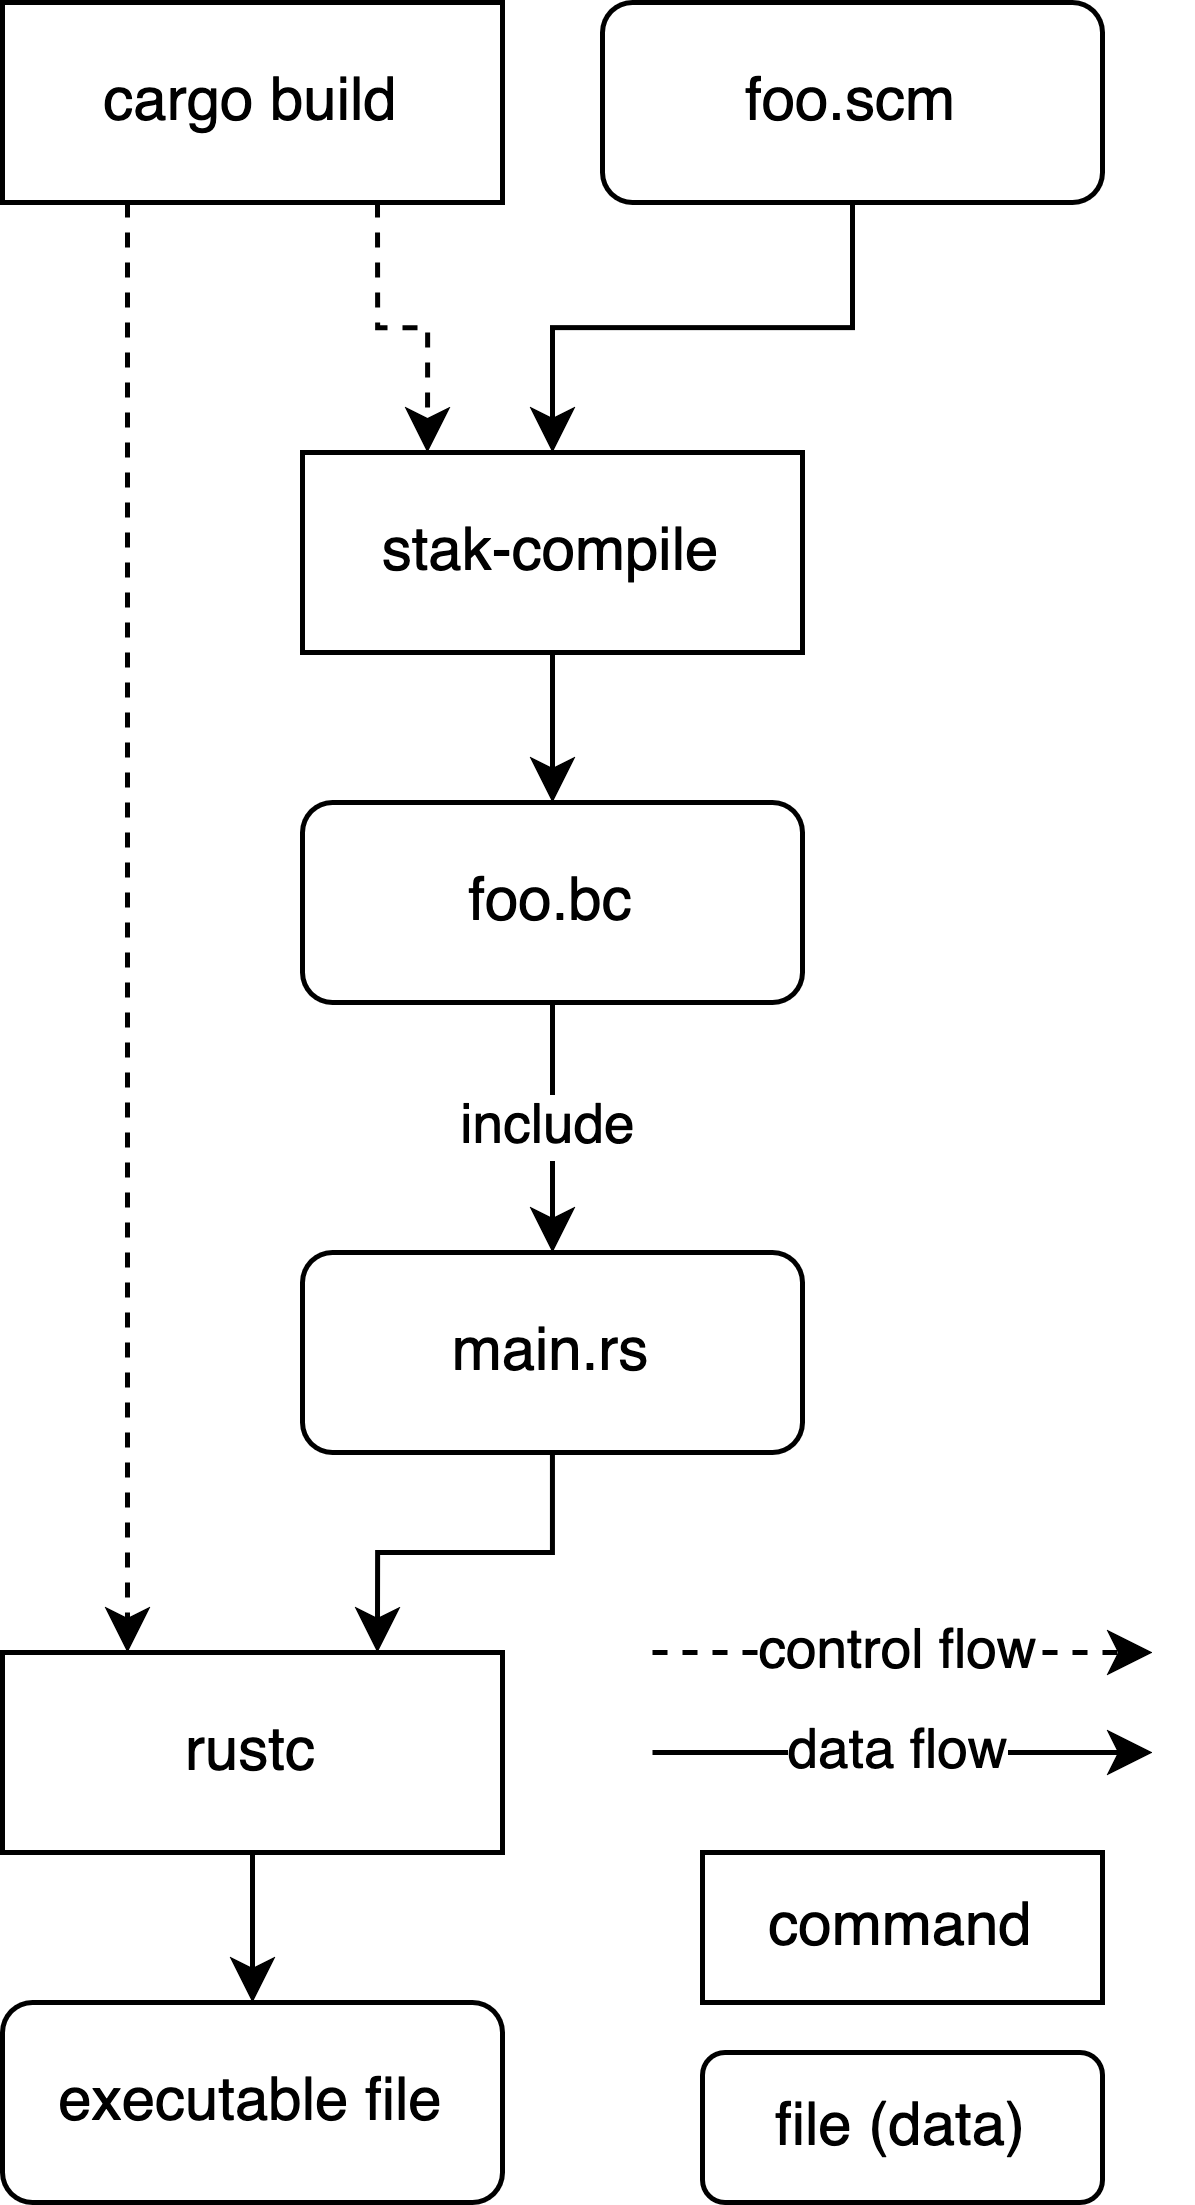
\includegraphics[width=0.35\textwidth]{build.png}
  \end{center}
\end{figure}

\begin{lstlisting}[float, caption=\texttt{foo.scm} file, label=list:scheme]
(import (scheme base) (scheme write))

(define (fibonacci x)
  (if (< x 2)
    x
    (+
      (fibonacci (- x 1))
      (fibonacci (- x 2)))))

(write (fibonacci 32))
\end{lstlisting}

\begin{lstlisting}[float, caption=Disassembled \texttt{foo.bc} file, label=list:bytecode]
...
constant procedure 1 #f
  get 0
  constant 2
  call 2 #f $<
  if
    get 0
  get 0
  constant 1
  call 2 #f $-
  call 1 #f fibonacci
  get 1
  constant 2
  call 2 #f $-
  call 1 #f fibonacci
  call 2 #f $+
call 1 #f $$close
set fibonacci
constant 32
call 1 #f fibonacci
call 1 #f write
\end{lstlisting}

\begin{lstlisting}[float, caption=\texttt{main.rs} file, label=list:rust]
fn main() -> Result<(), Box<dyn Error>> {
  // Include and run a Scheme module.
  run_scheme(&include_module!("foo.scm"))?;

  Ok(())
}

fn run_scheme(module: &UniversalModule)
    -> Result<(), EngineError> {
  // Initialize a heap memory for an engine.
  let mut heap = [Default::default(); HEAP_SIZE];
  // Initialize the engine.
  let mut engine = Engine::new(&mut heap, &mut [])?;

  // Finally, run the Scheme module in the engine.
  engine.run(module)
}
\end{lstlisting}

\subsection{Compiler} \label{compiler}

The bytecode compiler of Stak Scheme compiles source files in Scheme
into bytecode.
The Scheme script of the compiler is compatible with any R7RS-small
implementations including Stak Scheme itself for the purpose of bootstrapping.
In the current implementation, a single Scheme file of 1.5 KLOC
contains the whole bytecode compiler.

The compiler is composed of the following stages.

\begin{enumerate}
  \item Source code parsing
  \item Compiler inception
  \item Library expansion
  \item Macro expansion
  \item Compilation
  \item Bytecode marshalling
  \item Bytecode encoding
\end{enumerate}

First, we parse source code as S-expressions from source
files skipping whitespace characters and comments.
Then, in the stage of compiler inception, we \textit{incept} the compiler
itself into the source code, which is described in details later in
Section \ref{inception}.
In library and macro expansions, we expand library and macro
syntaxes, such as \texttt{define-library}, \texttt{import},
\texttt{define-syntax}, and \texttt{syntax-rules} in the source code.
Following the specification of the library system in the R7RS-small
standard, we need to segregate environments of different libraries.
We represent such environments by creating symbols from
different environments with the non-standard
\texttt{string->uninterned-symbol} procedure.
If the procedure is not available in the compiler host, we emulate
the procedure by prepending unique prefixes to symbols' string
representations.
The hygienic macro system is the implementation of the
algorithm described in Macros That Work \cite{macrosthatwork}.

The compilation phase compiles the expanded expressions to
bytecode in its in-memory format. Note that we use the same
in-memory format of the bytecode on our virtual machines as well.
Hence, we can reuse the
compilation logic inside the \texttt{(scheme eval)} library as it is
as well as the logic of library expansion and macro expansion.
We describe further details about how we reuse the compiler and build
the \texttt{(scheme eval)} library in Section \ref{inception}.

Before encoding bytecode, we marshal them for the following purposes:

\begin{itemize}
  \item We marshal immediate values of certain data types in bytecode
    instructions into their serializable representations.
  \item We make boxed values of certain data types, such as strings and
    characters, unique in bytecode so that we process them only once
    in the later bytecode encoding and reduce resulting bytecode sizes.
  \item We strip out string representation of symbols that are never used
    at runtime.
\end{itemize}

About the first item, to make the compiler compatible with any R7RS-small
implementations but not only Stak Scheme, we marshal immediate values
inside bytecode instructions into their "universal"
representations compatible with any R7RS-small hosts that emulate
the data representations in our virtual machines
described later in Section \ref{vm}.
For example, we represent a string as a tuple of its length, a list of
character code points, and a tag for the string type in the compiler,
which is expressed as a pair of the length and the list
with a pointer tag on the \texttt{cdr} side in the virtual
machines of Stak Scheme.

Finally, the bytecode encoding phase encodes the in-memory representation of
bytecode into its serialized format and write them into output files.
We discuss the details of bytecode encoding in \ref{encoding}.

\subsection{Virtual machine} \label{vm}

Stak Scheme's virtual machine is designed after the one of Ribbit
Scheme, Ribbit Virtual Machine (RVM).
Therefore, they share the large part of their design.
For example, both Ribbit and Stak Scheme's virtual machines represent
code and data as graphs of pair-like data structures in heap memory.
They initialize virtual machines by decoding bytecode onto
their heap memory.
However, we have several differences in instructions, Scheme value
representation, and bytecode.

First, while \texttt{constant}, \texttt{get}, \texttt{set}, and
\texttt{if} instructions in Stak Scheme are nearly identical to the ones in
Ribbit Scheme, the \texttt{call} instruction carries slightly
different semantics.
In Stak Scheme, the \texttt{call} instructions
contain function call signatures of arities and
flags indicating whether the function calls are variadic or not.
This arity information is used to align argument and parameter counts and
resolve the \textit{rest} parameters comparing it with signatures of
called procedures.
Thus, Stak Scheme does not have any \texttt{apply} primitive
procedure unlike Ribbit Scheme either.

Secondly, while Ribbit Scheme's virtual machine uses Ribs, triplets of
word-sized fields for internal representation of Scheme values, Stak
Scheme represents them as a traditional pair data structure of two
word size with optional tags attached to pointers in \texttt{cdr}.
This design choice simply saves a third of heap memory on the virtual machines
compared to Ribbit Scheme while it requires extra bit operations to
extract cons pointers and tags.
We use the optional pointer tags to encode instruction
codes or underlying data types primarily.
As well as Ribbit Scheme, we have only two primitive data types on virtual
machines; numbers and cons's.
Numbers are literally internal representations of mathematical numbers.
We currently provide three number
representations of 63-bit integers, 64-bit floating-point numbers,
and a mixture of 63-bit integers and 62-bit floating-point numbers
via Float Self-Tagging \cite{floatselftag}.
They are exclusive with each other and developers choose one
of the number representations when compiling the virtual machines.
Cons's are pairs of two primitive values and represented as
pointers into heap memory on the virtual machines.
In our Rust implementation of the virtual machine, we use an array of
primitive values as heap memory and indices into the array as cons
pointers.
In other implementations of the virtual machines, we can still fall
back to the data structures of Ribs where we allocate another
word-sized field for the tags if pointer tags are not available.

There is a subtle trick in our representation of Scheme values.
As we shrink down Ribs of triplets into traditional pairs, we sometimes
have no space to store data types as pointer tags anymore.
For example, how do we store the information that a value represented
by \texttt{(cons 1 2)} has the pair type?
The answer is that we assume tag values for numbers to be 0 which is of
the pair type
and store cons values in \texttt{cdr} for every other data type.
The internal representations of data types in Stak Scheme are listed
in Table \ref{table:types}.

\begin{table*}
  \begin{center}
    \caption{Internal representation of Scheme values}
    \label{table:types}
    \begin{tabular}{lll}
      \hline
      Type & car & cdr \\
      \hline
      Pair & number or cons & number or cons \\
      Null & number & cons \\
      Boolean & number or cons & cons \\
      Procedure & cons (environment) & cons (signature and code) \\
      String & number (length) & cons (code points) \\
      Symbol & number or cons (value of global variable) & cons
      (string representation) \\
      Character & number (code point) & cons (null) \\
      Vector & number (length) & cons (elements) \\
      Bytevector & number (length) & cons (bytes) \\
      Record & cons (metadata) & cons (fields) \\
      \hline
    \end{tabular}
  \end{center}
\end{table*}

Currently, we provide the implementation of the virtual machine only
in Rust.
However, as well as RVM, we believe that we can implement Stak Scheme's
virtual machine in different programming languages from low-level to high-level.
Besides, we do not assume linear memory on virtual machines in such
host languages of virtual machines.
Developers can also utilize garbage collectors of
the host languages in implementations of the virtual machine.
We discuss this topic in Section \ref{portvm} as future work further.

In Section \ref{bytecode}, we describe the bytecode format for the
virtual machine and its encoding and decoding algorithms in details.

\subsection{Bytecode} \label{bytecode}

Stak Scheme's bytecode represent programs for the virtual machines to
execute.
As described in Section \ref{vm},
we represent both code and data of instructions and immediate
values inside them in pair data structures consisting of two fields of
\texttt{car} and \texttt{cdr}.
Therefore, the problem of encoding and decoding bytecode falls into
the one on graphs of the pairs.
Furthermore, the graphs generated by the compiler are guaranteed to be
Directed Acyclic Graphs (DAGs), which even simplifies the encoding
and decoding.

While we provide only the Rust implementation of the virtual machine,
we keep the serialized format of bytecode portable across
different implementations of the virtual machines in other languages.
As such, we do not use, for example, snapshots of linear
memories of the virtual machines onto which we expand bytecode as a
serialization format of bytecode.

\subsubsection{Encoding} \label{encoding}

We encode bytecode from its in-memory format into its serialized format in the
bytecode compiler.
We embed the serialized bytecode inside Rust programs for later
execution of them.
The serialized format of bytecode needs to be compact to save space in
resulting binaries, portable to be executable in different
implementations of the virtual machines, and performant so that we
decode them efficiently on the virtual machines.

For the bytecode encoding, we use an algorithm similar to topological
sort \cite{topologicalsort} with the following requirements.

\begin{itemize}
  \item We have different data types of immediate values in instructions,
    such as numbers, nulls, booleans, strings, symbols, and so on.
    Expectantly, we encode values of most of the data types without
    introducing ad-hoc encoding rules for each data type.
  \item We encode values that are unique, such as symbols, in
    bytecode only once
    because they should have (surprisingly) only one instance.
    We also uniquify values of several other boxed data
    types in a prior pass of bytecode marshalling in the
    compiler discussed in Section \ref{compiler}.
    We should not duplicate the continuations of \texttt{if}
    instructions either but encode them only once to avoid the exponential bloat
    of the serialized bytecode \cite{ribbit7kb2023}.
  \item We do not use any complex data structures but only singly-linked lists
    during encoding to keep the decoding algorithm simple by its using
    only primitive data structures of numbers and cons's available on
    the virtual machines.
\end{itemize}

Algorithm \ref{algorithm:encode} describes an overview of the bytecode
encoding.
The $encode$ function encodes a given value of
underlying bytecode recursively where $I$ is an input of in-memory
bytecode to encode,
$O$ is an output of serialized bytecode, $C$ is a precomputed map of
reference counts
at which times each cons appears in the bytecode and $D$ is a
dictionary of \textit{shared} cons's represented as a list.

For each given value, we check if the value is a cons or not.
If not, we encode it as a number.
Otherwise, we check if the cons already exists in the dictionary $D$ of
shared values.
If so, we remove the value from the dictionary and push the value to
the top of the dictionary unless its reference count is zero.
Then, we encode the value's index in the dictionary $D$ and a flag of whether it
is removed from the dictionary or not into the output via the
$encodeIndex$ function.
The operation to move the values to the top of the dictionary is based on the
assumption of reference locality of such shared values in bytecode.
If the value is not in the dictionary $D$, we encode the child values in
\texttt{car} and \texttt{cdr} recursively as well as its tag.
Then, if its reference count is not zero, we push the shared value to
the top of the dictionary because it is the first time for the shared value
to appear in the bytecode.
Across the function, we track how many times the cons's appear and
decrement their counts every time when they show up in the bytecode.
When the counts of cons's reach zero, they are removed from the
dictionary $D$ as described above.
The $encodeCons$, $encodeNumber$, $encodeIndex$, and $encodePush$
functions write their corresponding decode instructions as byte
sequences to the output $O$.

\begin{algorithm}
  \caption{Bytecode encoding}
  \label{algorithm:encode}

  \KwIn{In-memory bytecode $I$}
  \KwOut{Byte sequence $O$}

  \Function{encode(x, O)}{
    \uIf{cons?(x)}{
      $c \gets getCount(C, x)$ \;
      \uIf{contain?(D, x)}{
        $i \gets position(D, x)$ \;
        $C \gets decrement(C, x)$ \;
        $D \gets remove(D, i)$ \;
        \If{c \neq 0}{
          $D \gets push(D, x)$ \;
        }
        $encodeIndex(i, c = 0, O)$ \;
      }
      \Else{
        $encode(car(x), O)$ \;
        $encode(cdr(x), O)$ \;
        $encodeCons(tag(x), O)$ \;
        $C \gets decrement(C, x)$ \;
        \If{c > 0}{
          $D \gets push(D, x)$ \;
          $encodePush(O)$ \;
        }
      }
    }
    \Else{
      $encodeNumber(x, O)$ \;
    }
  }

  $encode(I, O)$ \;
\end{algorithm}

\subsubsection{Decoding} \label{decoding}

We decode the serialized form of bytecode into heap memory on
our virtual machines.
The bytecode decoding in Stak Scheme happens by looking at each byte in
the serialized bytecode from the beginning to the end.
A chunk of bytecode for a Scheme program is a sequence of
variadic-length decode instructions of either $number$, $cons$, or $share$.

Algorithm \ref{algorithm:decode} describes an overview of the
bytecode decoding.
We initialize $I$ of an input with bytecode and $S$ of a stack for decoded
values and $D$ of a dictionary with empty lists.
The decoding starts with looking at the first byte in the bytecode.
If it is a $number$ instruction, we decode and push a number onto the stack.
If it is a $cons$ instruction, we decode a tag and construct a cons
from \texttt{car} and \texttt{cdr} values popped from the stack
and the tag to push it onto the stack.
If it is a $share$ instruction and of a \textit{push} operation, we push the
value at the top of a stack to the top of the dictionary.
Otherwise, we reference a shared value with its index in the
dictionary $D$ and push it onto the top of the stack.
Note that we also move the shared value to the top in the dictionary as well.
In addition, we remove the value from the dictionary if a flag $r$ is
true, which indicates that the value is not referenced anymore after the point.
Until we consume all the bytecode, we keep reading the decode instructions and
decode values.
Finally, the value at the top $car(S)$ is the root of the decoded
in-memory bytecode.

\begin{algorithm}
  \caption{Bytecode decoding}
  \label{algorithm:decode}

  \KwIn{Byte sequence $I$}
  \KwOut{In-memory bytecode $O$}

  $S \gets []$ \;
  $D \gets []$ \;
  \While{$I \neq []$}{
    $x \gets car(I)$ \;
    $I \gets cdr(I)$ \;
    \Switch{$instruction(x)$}{
      \uCase{$share$}{
        \uIf{$push?(x)$}{
          $D \gets cons(car(S), D)$ \;
        }
        \Else{
          $i, r, I \gets decodeIndex(x, I)$ \;
          \If{$i > 0$}{
            $d \gets tail(D, i - 1)$ \;
            $e \gets cdr(d)$ \;
            $cdr(d) \gets cdr(e)$ \;
            $D \gets cons(car(e), D)$ \;
          }
          $v \gets car(D)$ \;
          \If{$r$}{
            $D \gets cdr(D)$ \;
          }
          $S \gets cons(v, S)$ \;
        }
      }
      \uCase{$cons$}{
        $d \gets car(S)$ \;
        $S \gets cdr(S)$ \;
        $a \gets car(S)$ \;
        $S \gets cdr(S)$ \;
        $t, I \gets decodeCons(x, I)$ \;
        $S \gets cons(rib(a, d, t), S)$ \;
      }
      \Other{
        $n, I \gets decodeNumber(x, I)$ \;
        $S \gets cons(n, S)$ \;
      }
    }
  }

  $O \gets car(S)$ \;
\end{algorithm}

\subsection{Compiling the \texttt{eval} procedure} \label{inception}

The R7RS-small standard defines the \texttt{eval} procedure in the
\texttt{(scheme eval)} library, which evaluates arbitrary S-expressions in
arguments in specified evaluation environments.
In order to make the \texttt{eval} procedure fully-featured in Stak Scheme, we
ultimately need the full compiler we described in Section
\ref{compiler} inside the \texttt{(scheme eval)} library.

To realize that, we \textit{incept} the compiler itself into the
source code during the bytecode compilation.
In particular, the compiler script replaces
the \texttt{(\$\$compiler)} primitive call in the source code
with the compiler function right after the source code reading.
In the compiler script, we first define code of the compiler as
data stored in variables.
The compiler body is split into two parts.
The first part contains all the components required by the \texttt{eval}
procedure, such as the library system, the macro system, and the
bytecode compilation logic, that we embed into the source code.
The other half contains the other parts for the compiler, such
as bytecode marshalling and encoding logic.
In the main procedure of the compiler script, we combine the two
parts into one and apply the \texttt{eval} procedure against it to
run the whole compiler.

\section{Evaluation} \label{evaluation}

Our evaluation of Stak Scheme demonstrates the minimality of its design and
implementation as well as its reasonable performance compared with
other Scheme implementations and scripting languages.

\subsection{Lines of code}

To evaluate the compactness of our implementation of Stak Scheme,
we compare lines of code between our Stak Scheme implementation and
another small R7RS implementation, TR7 \cite{tr7}.
To the best of our knowledge, TR7 is the smallest R7RS implementation
among the ones written in Scheme and a certain system programming language.

To count lines of code, we exclude test code, comments, and blank
lines from source code in each implementation.
For Stak Scheme, there is no test code written in Scheme but only in Rust.
In the Rust code, we removed modules that are compiled only for tests.
In TR7, because it separates test code into different files, we simply did not
include such files.
Besides, we apply code formatters of \texttt{rustfmt} (v1.8.0),
\texttt{clang-format} (v20.1.7), and \texttt{schemat} (v0.4.1) for
Rust, C, and Scheme respectively.

As Table \ref{table:loc} shows, Stak Scheme almost
halves the code size compared to TR7.
One of the key factors is its split architecture of the bytecode
compiler in Scheme and the virtual machine in Rust.
As a result, we can write the large part of the language processor in Scheme
itself that is more abstract and high-level than Rust or C.
The small virtual machine design borrowed from Ribbit Scheme also
contributes to reduce the code size of its implementation in Rust.

\begin{table}
  \begin{center}
    \caption{Lines of code}
    \label{table:loc}
    \begin{tabular}{l|rrrrrrrr}
      \hline
      Language & Stak & TR7  \\
      \hline
      Scheme & 3792 & 116 \\
      C / Rust & 5878 & 16775 \\
      Total & 9670 & 16891 \\
      \hline
    \end{tabular}
  \end{center}
\end{table}

Although both Stak Scheme and TR7 do not implement the complete
specification of R7RS-small, we believe that the other
implementations would not be comparable with them since
Stak Scheme and TR7 implement all the primary language features,
such as library system and hygienic macros, already.
As adding missing functions or syntaxes are trivial changes,
implementing such additional functionalities would not change the
order of their lines of code.

\subsection{Computational benchmarks}

We compare interpreters of Stak Scheme, other R7RS-small Scheme
implementations, and
dynamic languages other than Scheme in computational
benchmarks shown in Table \ref{table:computation}.

The interpreters of Scheme and other languages we compare are not equipped with
any JIT compilation or other methods compiling the languages into
native code.
The following list is the versions and implementations of
the language interpreters used in the benchmarks.
For interpreters of non-Scheme dynamic languages, we choose CPython and
MRI Ruby in addition to their small implementations of MicroPython
and mruby, which are optimized against their binary sizes for
embedded scripting.

\begin{description}
  \item[tr7i] The TR7 interpreter at the commit \texttt{e821e555}
    on the \texttt{v2} branch
  \item[gsi] The interpreter of Gambit Scheme v4.9.5
  \item[chibi-scheme] Chibi Scheme v0.11
  \item[python3] CPython 3.13.3
  \item[micropython] MicroPython v1.25.0
  \item[ruby] MRI Ruby 3.4.4
  \item[mruby] mruby 3.4.0
\end{description}

For the benchmarks, we use the version of Stak Scheme that uses a
mixture of 63-bit integers and 62-bit floating-point numbers with Float
Self-Tagging \cite{floatselftag} as its number representation
for the sake of the better feature parity with
the other Scheme implementations while Stak Scheme does not implement
the full numeric tower defined in the R7RS-small standard.

The results in Table \ref{table:computation} indicates that Stak
Scheme's computational performance is still comparable with the other
Scheme implementations and dynamic languages at the range of 1.15
time faster to 2.33 time slower computation times
despite its minimal design and implementation.

\begin{table*}
  \begin{center}
    \caption{Computational benchmarks (relative time. lower is better.)}
    \label{table:computation}
    \begin{tabular}{l|rrrrrrrrr}
      \hline
      Benchmark & mstak & stak & tr7i & gsi & chibi-scheme & python3
      & micropython & ruby & mruby \\
      \hline
      fibonacci & 1.00 & 1.06 & 1.03 & 1.11 & 0.82 & 0.50 & 1.15 &
      0.55 & 0.67 \\
      sum & 1.00 & 1.10 & 0.92 & 1.01 & 0.80 & 0.61 & 0.48 & 0.59 & 0.86 \\
      tak & 1.00 & 1.03 & 0.80 & 0.84 & 1.09 & 0.43 & 0.91 & 0.59 & 0.52 \\
      \hline
    \end{tabular}
  \end{center}
\end{table*}

\section{Related work}

Ribbit Scheme \cite{ribbit2023} is the tiny and portable R4RS Scheme
implementation we designed Stak Scheme after. They provide
Ribbit Virtual Machines (RVMs) in various programming languages
including x86-64 assembly, C, JavaScript, Bash, Scheme, etc.
They have first coined the basic architecture of Ribbit Scheme
\cite{ribbit2021} where its implementation is composed of an
Ahead-Of-Time (AOT) bytecode compiler and a tiny virtual machine.
The AOT compiler compiles source code in Scheme and produces
executable binaries bundled with virtual machines of specified backends.
This architecture allows users to strip unnecessary language
features and minimize resulting binaries.
In RVM, every code or data is represented in
Ribs, which are tuples of three fields.
That does not only make the implementation of
virtual machines simple but make them portable across different
programming languages from low-level to high-level.

Although Ribbit Scheme's bytecode encoding is very efficient
for small Scheme programs already,
Stak Scheme's encoding algorithm deviates quite a bit to encode and decode
large chunks of bytecode.
First, the bytecode encoding of Ribbit Scheme requires a global symbol table.
Because this table is used for both global variables and cache of
boxed constant values, we suffer from the larger and larger global tables
as we grow the size of source programs and standard libraries.
When we self-host our fairly large bytecode compiler in Stak Scheme,
the performance degrade makes builds of Scheme programs painful due
to lengthy build times.
As we discussed in Section \ref{encoding}, we take another approach that
does not require any global symbol table.
Secondly, Ribbit Scheme's bytecode encoder encodes instructions
with immediate values of only primitive data types.
To encode complex data structures in the bytecode, the encoder
generates bytecode to initialize such values attached at the
beginning of the programs.
In Stak Scheme, we instead encode instructions and their immediate
values uniformly as graphs of pair data structures even when the
immediate values are not of primitive data types.
Our preliminary experiments shows speedup of startup
latencies of Scheme programs at the sacrifice of compact bytecode
increasing their sizes in bytes.

TR7 \cite{tr7} is the tiny R7RS Scheme implementation written in C.
The key differences between Stak Scheme and TR7 are primary languages used in
the implementation and how they strip out features from the
interpreters.
TR7 intentionally uses only C for most part of its implementation and
contains its entire interpreter in one \texttt{tr7.c} source file and a
\texttt{tr7.h} header file whereas Stak Scheme uses both Scheme and
Rust for its bytecode compiler and virtual machine.
TR7 allows users to strip language features from the interpreter via
the C preprocessor macros prefixed with \texttt{USE\_}.
On the other hand, Stak Scheme allows users to strip out the majority of
the interpreter logic, such as S-expression parsing, library system, and
macro expansion, from resulting binaries in its bytecode compiler
depending of libraries given source programs import.

\section{Future work}

\subsection{Type checking and virtual machine memory safety}

One of the reasons why Stak Scheme is tiny and its performance is still
comparable with the other Scheme implementations is that its
programs are not memory safe on the virtual machines even though
the host language is memory safe.
The programs written in Stak Scheme are able to access any memory
locations on the virtual machines as long as the host languages allow that.
In the virtual machine we implemented in Rust, this memory
unsafety on virtual machines sometimes arises as panics with little
contextual information.
Such panics are hard to debug, especially when debug information is
stripped out from executable files of the interpreter.
We have a plan to implement basic type checks in our virtual machine
in the host language of Rust in order to enhance memory safety on
the virtual machine without sacrificing its performance.

\subsection{Tree shaking}

One of methods to reduce the size of programs in dynamic programming
languages is tree shaking\cite{treeshaking}, which is commonly used
in bundlers of JavaScript, such as Webpack \cite{webpack} and Rolldown
\cite{rolldown}.
Tree shaking "shakes down" unnecessary code from
the whole programs with checks of visibility and side effects.
Although dead code elimination is a commonly known pass in the
compiler technology, the term of tree shaking is used
in the context of dynamic programming languages where we do not define
any entrypoint functions.
When we implement it in Stak Scheme, tree shaking would not only
reduce the size of bytecode but also decrease the startup latencies
because it reduces time for bytecode decoding on virtual machines.
Since we expand libraries and macros statically
in our bytecode compiler, we believe that it is relatively easy to
implement tree shaking compared with other implementations of Scheme
where, for example, the \texttt{define-syntax} syntax is defined as a macro.

\subsection{Porting virtual machines to other languages} \label{portvm}

Although we believe that our bytecode decoding algorithm work
universally across different host languages, we did not implement them in
virtual machines written in programming languages other than Rust yet.
For the first step, we have a plan to implement another virtual
machine in the Go programming language, which is another memory-safe system
programming language widely used today.
As Go comes with its own garbage collector,
it would be intriguing to evaluate how well its implementation of the
virtual machine performs compared with the virtual
machine with copy garbage collection in Rust.
Porting the Stak Scheme virtual machine to other languages does
not only prove its portability but also extends its use cases.

\section{Conclusion}

Stak Scheme is a tiny R7RS-small implementation written in Scheme and
Rust.
Although our implementation of Stak Scheme is minimal in terms of
lines of code, it still demonstrates reasonable performance.
Our evaluation shows that Stak Scheme is
comparable with the other Scheme implementations and dynamic
programming languages in terms of computational time performance.

We plan to further improve the design and implementation of Stak
Scheme in the future. The upcoming work includes but is not limited
to type checking, tree shaking, and porting the virtual machine to
another system programming language.

\begin{acks}
  We cannot thank enough the dynamic programming language team at
  Montreal university, Canada for the foundational work of Ribbit
  Scheme, which heavily inspired the design and implementation of
  Stak Scheme.
\end{acks}

\bibliographystyle{ACM-Reference-Format}
\bibliography{references}

\end{document}
